\section{Evaluation}

In this section we provide two evaluation of the proposed mehtod.
First we show with the example of the circadian clock model of \cite{comet2012simplified} that our method can re-construct the correct $PH$ from its observations.
Here the model is known and we generate the corresponding chronogram given from an initial state.
We evaluate the capacity of our algorithm\footnote{All programs, described in this article, for PH generation and for the refinement are implemented in Answer Set Programming (ASP) and are available online at: \url{http://git.irccyn.ec-nantes.fr/benabdal/generate_revise_d-brn/repository/archive.zip}} to find the correct actions and the impact of the quantity of observations on run time.
In the second experiment our goal is to assess the scalability of our approach in practice.
Here we process chronograms obtained from time series data of the DREAM4 challenge \cite{prill2011crowdsourcing}.

% Evaluation de la méthode de la completion/revision des PH
\label{sec:evaluation}
\subsection{Circadian clock}

In this section, we evaluate our approach on learning the circadian clock actions.
These experiments are run on a processor Intel Xeon (X5650, 2.67GHz) with 12GB of RAM.

	\begin{figure}[htb!]\centering
	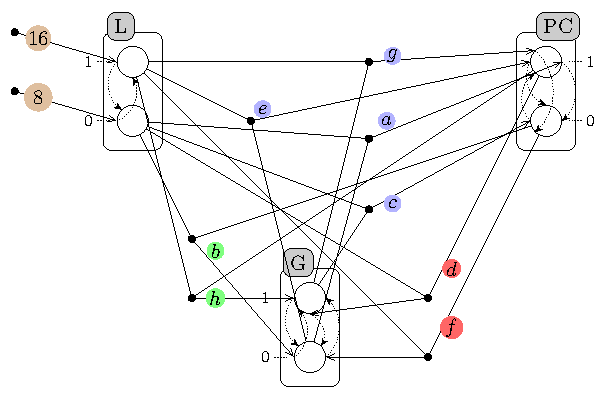
\includegraphics[width=0.45\linewidth]{images/circadianPH.pdf}
	%
	\hspace{0.1cm}
	%
	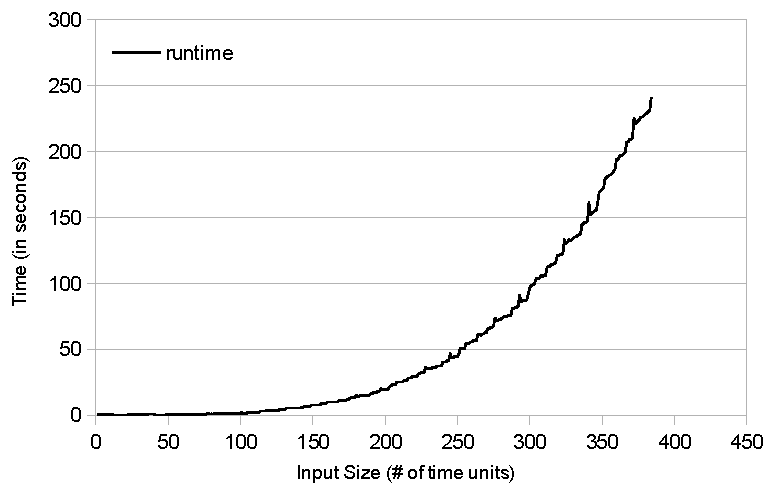
\includegraphics[width=0.45\linewidth]{images/circadian_run_time}
	\label{fig:PH_circadian}
	\caption{Representation of circadian clock in Process Hitting (left). The value $"a", "b", ..., "h"$ represent the delays in actions.
	Run time of the application of Algorithm \ref{alg:PHG_ap} on circadian clock chronograms varying the number of time steps (right)}
	
	\label{fig:run_time}	
	\end{figure}
%

Figure \ref{fig:run_time} shows the evolution of run time of our ASP implementation of Algorithm \ref{alg:PHG_ap} on the inference of the circadian clock actions regarding the quantity of input data.
In this experiment, our algorithm succeed to learn the correct actions.
Using this benchmark we also analysed the scalability of our approach by varying the number of time units of the input, \ie the size of the chronogram.
Here we can see that the time needed to analyse the input data grows exponentially.
The experiments stop at $384$ because the memory required by the ASP solver reached the 12GB of RAM we have.
It is currently quite difficult to obtain real data from biological system with chronogram exceeding 100 points.
In work like \cite{Fippo14} the considered chronograms are only composed of about 10 points.
Regarding the circadian clock, a chronogram of 100 data points is about 4 days of data, that is not much information, especially in cases where we want to analyze the effect of perturbations (for example, understand the recoverability phase in case of jet-lag). 

\subsection{DREAM4}
	
	In this section, we assess the efficiency of our algorithm through case studies coming from the DREAM4 challenge.
	DREAM challenges are annual reverse engineering challenges that provide biological case studies.
	In this paper, we focus on the datasets coming from DREAM4.
	The input data that we tackle here consists of the following:
	5 different systems each composed of 100 genes, all coming from E. coli and yeast networks. For every such system,
	the available data are the following: (i) 10 time series data with 21 time points and 1000 is the duration of each time series; (ii) steady state for wild type;
	(iii) steady states after knocking out each gene;
	(iv) steady states after knocking down each gene (i.e. forcing its transcription rate at 50\%);
	(v) steady states after some random multifactorial perturbations. We processed all the data.
	Here, we focus on the management of time series data.\\
	%
%\subsection{Settings}
	%
	Each time serie includes different perturbations that are maintained all time along during the first 10 time points and applied to at most 30 genes.
	In this setting, a perturbation means a significant increase or decrease of the gene expression.
	%
	In the raw data of the time series, gene expression values are given as real numbers between 0 and 1.
	To apply our approach, we chose to discretize those data into two to six qualitative values.
	Each gene is discretized in an independent manner, with respect to the following procedure:
	we compute the average value of the gene expression among all data of a time series,
	then the values between the average and the maximal/minimal value are divided into as many levels.
	Discretizing the data according to the average value of expression is expected to reduce the impact of perturbation on the discretization and thus on the model learned.
	But in this experiment our goal is to assess the scalability of our approach in practice rather than evaluating the model learned when facing perturbated data.
	Figure \ref{fig:run_time} shows the impact of both actions indegree and discretization level on run time.

%\subsection{Results}

	\begin{figure} \centering
	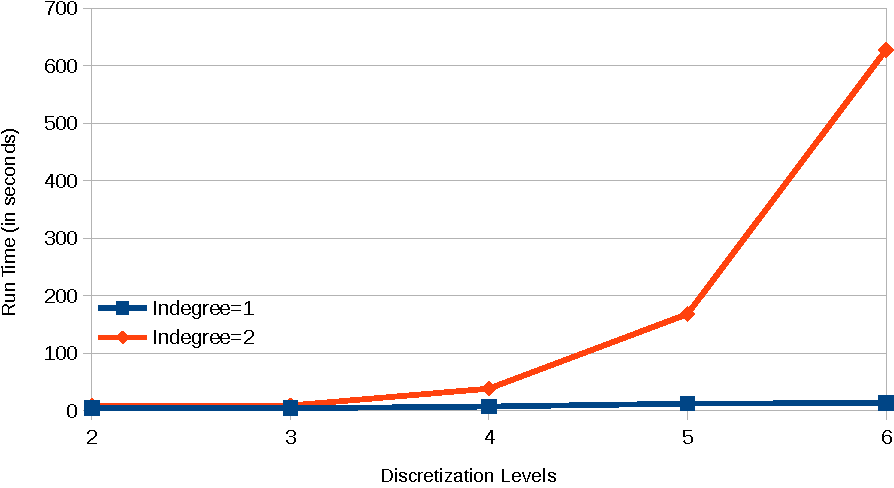
\includegraphics[width=0.32\linewidth]{images/net1}
	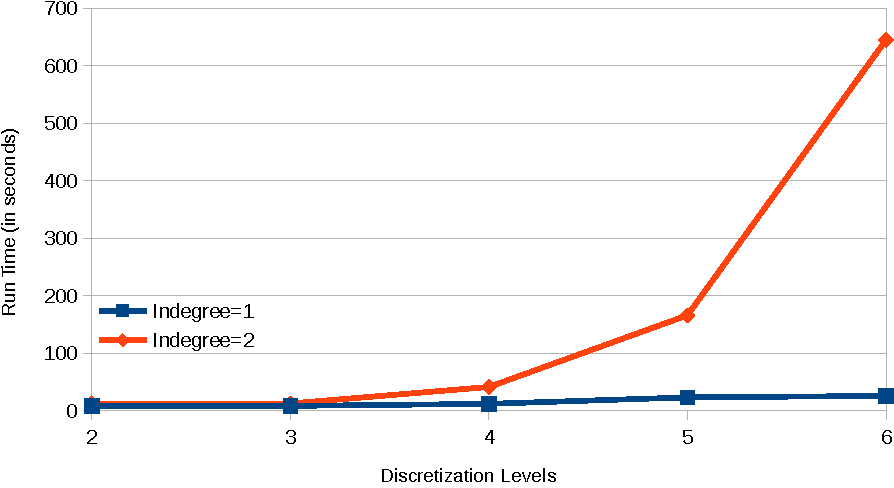
\includegraphics[width=0.32\linewidth]{images/net2}
	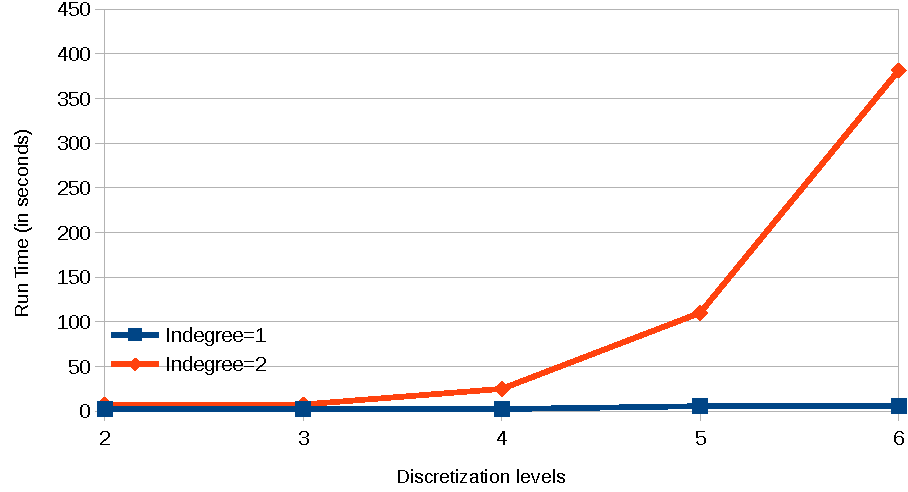
\includegraphics[width=0.32\linewidth]{images/net3}
	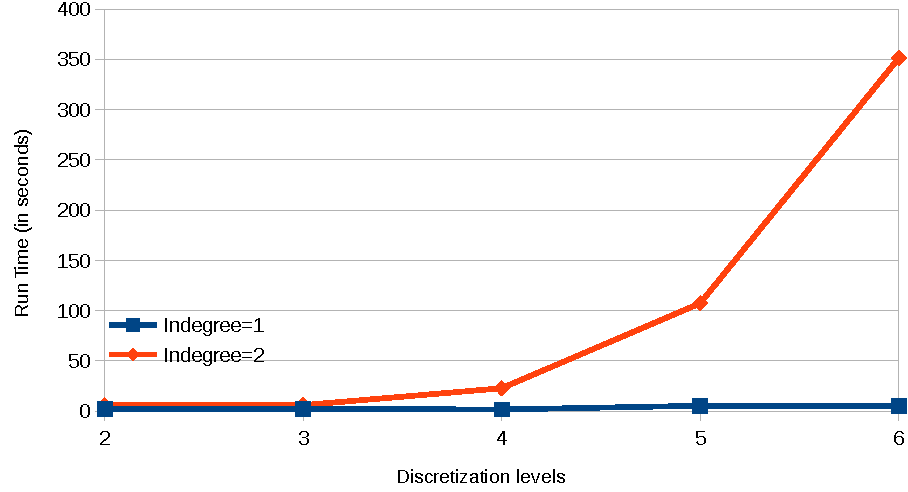
\includegraphics[width=0.33\linewidth]{images/net4}
	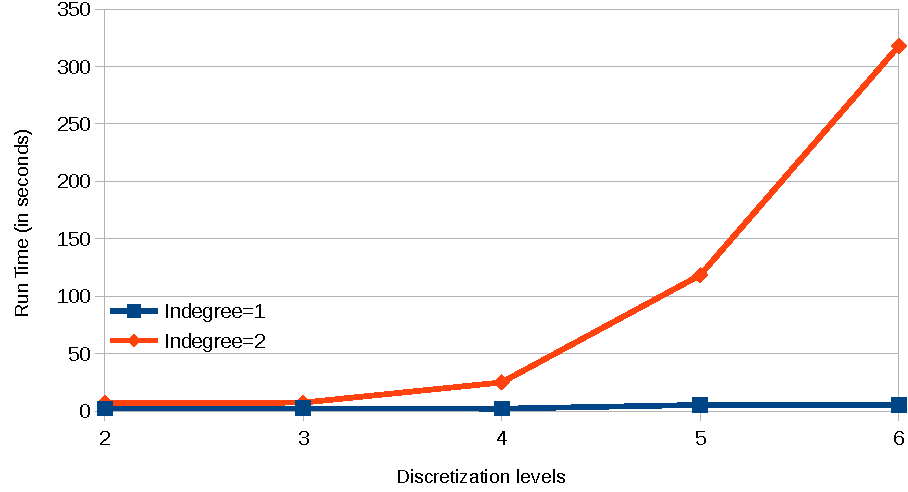
\includegraphics[width=0.33\linewidth]{images/net5}
	\label{fig:run_time}
	\caption{Evolution of run time on processing different model time series data from DREAM4 varying indregree of actions and discretization levels. These tests were performed on processor: 3 GHz Intel Core i7 with 16 Go of RAM. }
	\end{figure}

	In the results obtained from the experimentations of our algorithm on the time series data of the DREAM4 we can see the exponential influence on the run time of indegree of action considered as well as the level of discretization chosen for all the 5 different networks.
	But it also shows that in practice our approach can tackle big network, here 100 genes.
	It is important to note that here the real influences are given as background knowledge, 
	thus it greatly reduces the quantity of action generated to explain each change.
	Without knowledge about those influences, the algorithm can be run considering that all genes can be influenced by all other genes.
	But here, the quantity of combination of influences is so huge that processing only one time series discretized into two levels of expression with an indegree of two takes more that 12 hours to process. In practice, on large networks (more than 40 genes), accessing to information about genes influences is crucial for the efficiency of this method.
	
%	The current version does not provide guaranty about the soundness of the model learned.
%	More practical study of the method is required to design methods to provide guaranty about output.
	
	
	
%\textcolor{red}{COMMENT Tony: Faudrais testé en augmentant le nombre de time points si possible. Egalement avec un indegree de 3, 4 jusqu'a ce que ça soit trop long.}
